\section{Informe sobre la clase \texttt{Picture}}

La clase \texttt{Picture} en el código presentado está diseñada para manejar y manipular imágenes representadas como listas de cadenas de caracteres. Esta clase ofrece diversas funcionalidades para transformar y combinar imágenes de diferentes maneras. A continuación, se presenta un análisis detallado de sus métodos y atributos.

\subsection{Atributos}

\begin{itemize}
    \item \texttt{img}: Este atributo almacena la imagen, que es una lista de cadenas de caracteres donde cada cadena representa una fila de la imagen.
\end{itemize}

\subsection{Métodos}

\begin{enumerate}
    \item \textbf{Constructor (\texttt{\_\_init\_\_})}
    \begin{lstlisting}
    def __init__(self, img):
        self.img = img
    \end{lstlisting}

    \item \textbf{Igualdad (\texttt{\_\_eq\_\_})}
    \begin{lstlisting}
    def __eq__(self, other):
        return self.img == other.img
    \end{lstlisting}

    \item \textbf{Invertir Color (\texttt{\_invColor})}
    \begin{lstlisting}
    def _invColor(self, color):
        if color not in inverter:
            return color
        return inverter[color]
    \end{lstlisting}

    \item \textbf{Espejo Vertical (\texttt{verticalMirror})}
    \begin{lstlisting}
    def verticalMirror(self):
        vertical = []
        for fila in self.img:
            espejo = ""
            for letra in fila:
                espejo = letra + espejo
            vertical.append(espejo)
        return Picture(vertical)
    \end{lstlisting}

    \item \textbf{Espejo Horizontal (\texttt{horizontalMirror})}
    \begin{lstlisting}
    def horizontalMirror(self):
        horizontal = []
        for i in range(len(self.img)):
            l = len(self.img) - i - 1
            horizontal.append(self.img[l])
        return Picture(horizontal)
    \end{lstlisting}

    \item \textbf{Negativo (\texttt{negative})}
    \begin{lstlisting}
    def negative(self):
        new_img = []
        for string in self.img:
            new_string = [self._invColor(letter) for letter in string]
            new_img.append(new_string)
        return Picture(new_img)
    \end{lstlisting}

    \item \textbf{Unir (\texttt{join})}
    \begin{lstlisting}
    def join(self, p):
        new_img = []
        l = max(len(self.img), len(p.img))
        for i in range(l):
            izquierda = self.img[i] if i < len(self.img) else [" " for _ in range(len(self.img[0]))]
            derecha = p.img[i] if i < len(p.img) else [" " for _ in range(len(p.img[0]))]
            row = "".join(izquierda) + "".join(derecha)
            new_img.append(row)
        return Picture(new_img)
    \end{lstlisting}

    \item \textbf{Colocar Arriba (\texttt{up})}
    \begin{lstlisting}
    def up(self, p):
        new_img = self.img + p.img
        return Picture(new_img)
    \end{lstlisting}

    \item \textbf{Colocar Debajo (\texttt{under})}
    \begin{lstlisting}
    def under(self, p):
        new_img = p.img + self.img
        return Picture(new_img)
    \end{lstlisting}

    \item \textbf{Repetición Horizontal (\texttt{horizontalRepeat})}
    \begin{lstlisting}
    def horizontalRepeat(self, n):
        new_img = []
        for row in self.img:
            new_row = row * n
            new_img.append(new_row)
        return Picture(new_img)
    \end{lstlisting}

    \item \textbf{Repetición Vertical (\texttt{verticalRepeat})}
    \begin{lstlisting}
    def verticalRepeat(self, n):
        new_img = self.img * n
        return Picture(new_img)
    \end{lstlisting}

    \item \textbf{Rotar en Sentido Horario (\texttt{rotate\_horario})}
    \begin{lstlisting}
    def rotate_horario(self):
        transpuesta = list(zip(*self.img))
        rotada = [list(fila)[::-1] for fila in transpuesta]
        return Picture(rotada)
    \end{lstlisting}

    \item \textbf{Rotar en Sentido Antihorario (\texttt{rotate\_antihorario})}
    \begin{lstlisting}
    def rotate_antihorario(self):
        return self.rotate_horario().rotate_horario().rotate_horario()
    \end{lstlisting}

    \item \textbf{Superposición (\texttt{on})}
    \begin{lstlisting}
    def on(self, p):
        new_img = []
        for i in range(len(self.img)):
            row = self.img[i]
            p_row = p.img[i]
            new_row = []
            for j in range(len(row)):
                if row[j] == " ":
                    new_row.append(p_row[j])
                else:
                    new_row.append(row[j])
            new_img.append(new_row)
        return Picture(new_img)
    \end{lstlisting}

    \item \textbf{Métodos Estáticos para Crear Piezas}
    \begin{lstlisting}
    @staticmethod
    def rock():
        return Picture(ROCK)

    @staticmethod
    def king():
        return Picture(KING)

    @staticmethod
    def bishop():
        return Picture(BISHOP)

    @staticmethod
    def square():
        return Picture(SQUARE)

    @staticmethod
    def knight():
        return Picture(KNIGHT)

    @staticmethod
    def pawn():
        return Picture(PAWN)

    @staticmethod
    def queen():
        return Picture(QUEEN)
    \end{lstlisting}
\end{enumerate}

\section{Ejercicios con la biblioteca}
Las figuras que se nos pidio hacer son:

\begin{figure}
    \centering
    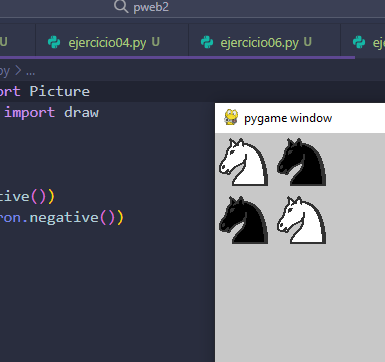
\includegraphics[width=0.5\linewidth]{1.png}
    \caption{1}
    \label{fig:enter-label}
\end{figure}

\begin{figure}
    \centering
    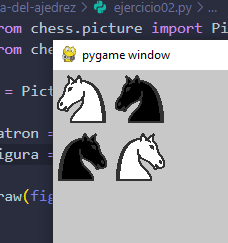
\includegraphics[width=0.5\linewidth]{2.png}
    \caption{2}
    \label{fig:enter-label}
\end{figure}

\begin{figure}
    \centering
    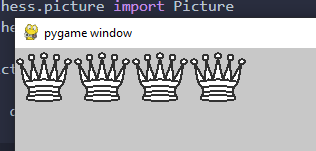
\includegraphics[width=0.5\linewidth]{3.png}
    \caption{3}
    \label{fig:enter-label}
\end{figure}

\begin{figure}
    \centering
    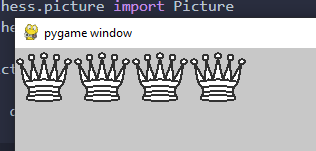
\includegraphics[width=0.5\linewidth]{4.png}
    \caption{4}
    \label{fig:enter-label}
\end{figure}

\begin{figure}
    \centering
    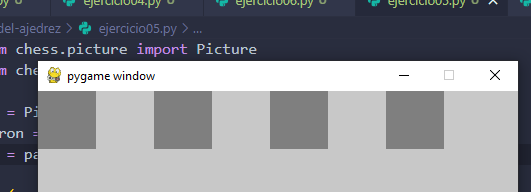
\includegraphics[width=0.5\linewidth]{5.png}
    \caption{5}
    \label{fig:enter-label}
\end{figure}

\begin{figure}
    \centering
    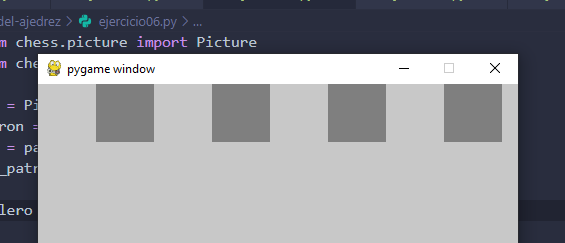
\includegraphics[width=0.5\linewidth]{6.png}
    \caption{6}
    \label{fig:enter-label}
\end{figure}

\begin{figure}
    \centering
    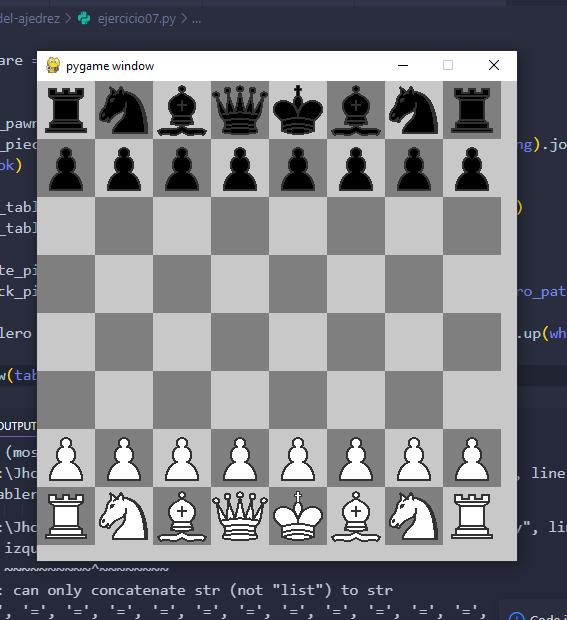
\includegraphics[width=0.5\linewidth]{7.png}
    \caption{7}
    \label{fig:enter-label}
\end{figure}

\section{Pregunta}
El directorio pycache es para guardar las instancias de las calses para cposterior consulta